%% ============================================================================
\section{LoCoBench: Data and Full Results}
\label{sec-full-locobench}
\label{app:results}
%% ============================================================================

\subsection{The Data in Brief}

\citet{anonlocobench} describe how LoCoBench is built and validated; we summarize what the
evaluation relies on. Table~\ref{tab:lb-ladders} lists the five ladder types. A generator (Claude
Opus~5) writes a question, a pool of claims with factuality labels (a few plausible but false), a
plan that fixes the relations and slots, and a template with the fillers of every slot. A
deterministic gate checks, before any prose is written, that each ladder's gold graphs are ordered
in the coherence order at the verdicts, with a step of at least $0.05$ nats in $\Lambda$ between
neighbouring rungs. A committee of three models from three vendors (GPT-6.1, Gemini~3.1 Pro and
Claude Opus~5.5) admits a template only if a majority rates it fluent and free of annotation
leakage, finds every claim asserted, and confirms its relations pair by pair without seeing the
plan. It admits a filler only if a majority, not told which link was intended, reads exactly that
link. Where the committee's reading of a fixed relation departs from the plan, gold follows the
reading. The \sThreeItems{} responses carry 10,636 gold relations, 8,078 with a factor, of which
6,767 are supports and 1,311 conflicts at the verdicts.

\begin{table*}[t]
\centering\small
\setlength{\tabcolsep}{4pt}
\begin{tabular}{@{}lp{3.6cm}p{6.8cm}l@{}}
\toprule
Ladder & Slots & Rungs $\rho_0\to\rho_1\to\rho_2$ & Declared \\
\midrule
\cp{conflict} & two (plus a spare), each joining two true claims
  & both slots assert that their claims cannot both hold; one does; neither does & increasing \\
\cp{chain} & two consecutive links $p\to p{+}1\to p{+}2$ between true claims
  & neither link drawn; the first drawn; both drawn & increasing \\
\cp{sign} & one (plus a spare) joining a true claim to a false one
  & the falsehood derived from the truth; no link; the falsehood refuted by the truth & increasing \\
\cp{order} & none & three paragraph orders of self-contained paragraphs & invariant \\
\cp{control} & one, an entailment between true claims & three wordings of the same link & invariant \\
\bottomrule
\end{tabular}
\caption{The five ladder types. Every family has one primary ladder (\cp{conflict}, \cp{chain},
\cp{sign} or \cp{order}) and a \cp{control} ladder on one extra slot, whose $\rho_0$ is the
primary ladder's $\rho_1$; a family therefore has five distinct responses. Declared orders are at
verdict polarity; only \cp{sign}'s changes under assertion polarity.}
\label{tab:lb-ladders}
\end{table*}


\paragraph{What admission does and does not select.} The committee confirms relations with a
blind pair-by-pair verification, not with the open recovery prompt our graph-level miner uses, so
admission no longer selects for what that miner recovers. Two dependencies remain. The gold
graphs are what the committee read, so mined results measure agreement with that reading; and the
committee and the miners share vendors (GPT-6.1 on the committee, GPT-6 and gpt-oss among the
miners), although no model is both. Because the fillers are written to be explicit, the
ladders test whether a score orders responses whose relations differ, not how often such
differences arise in practice.

\subsection{Setup Details}
\label{app:setup-details}

\paragraph{One score, two scales.} The score under evaluation is $\LCS$ (Def.~\ref{def:score}),
and ``LCS'' in every figure and table is that score. Its log-ratio form
$\Lambda=\log\PR(\xs)/\pi(\xs)$ (Eq.~\ref{eq:lambda}), in which the theorems are stated, is not a
second score but the same one on an unbounded scale: the rungs of a ladder share their claims and
flat priors, so $\pi(\xs)=2^{-n}$ on every rung, for the verdict world and the asserted world
alike, and $\LCS$ is a strictly increasing function of $\Lambda$ (App.~\ref{app:lcs-lambda}
plots the two scales side by side). The two therefore rank every rung pair identically, and
every count below of satisfied orderings, kept invariances and dominance classes holds for both.
Across all arms and both polarities the two never move in opposite directions
(\sThreeLamLcsSignDis{} of \sThreeLamLcsPairs{} rung pairs).

We use each scale for what it shows best. \emph{Whether} the score moves is decided on
$\Lambda$, in exact arithmetic with a resolution of $10^{-9}$. Near $0$ the logistic compresses
even large steps beyond any fixed resolution: on one pairwise-miner ladder the lowest rung has
$\LCS\approx10^{-17}$, and a step of $13$ nats in $\Lambda$ from it moves $\LCS$ by
$5\times10^{-12}$.
Taking the same decision on $\LCS$ would change nothing on gold graphs or on either graph-level
arm's graphs (\sThreeGoldLamLcsDis, \sThreeGraphGptLamLcsDis{} and \sThreeGraphOssLamLcsDis{}
rung pairs) but would turn
\sThreePairOssLamLcsDis{} and \sThreePairLlamaLamLcsDis{} of the pairwise arms' rung pairs into
ties. \emph{How far} the score moves, the tolerance $\tau$, resolved increases, saturation and
every plotted value, is read on $\LCS$'s $[0,1]$ scale, the scale a user of the score sees. Step
sizes quoted in nats are steps in $\Lambda$: a step of $\Delta$ nats multiplies the probability of
the committed world by $e^{\Delta}$, so $0.5$ nats is a factor of $1.65$ and $13$ nats a factor of
about $440{,}000$.

\subsection{Full Results}

\begin{table*}[t]
\centering\small
\setlength{\tabcolsep}{4.2pt}
\begin{tabular}{@{}lc ccc ccc@{}}
\toprule
& & \multicolumn{3}{c}{$\LCS$, assertion polarity}
& \multicolumn{3}{c}{$\LCS$, verdict polarity (ours)} \\
\cmidrule(lr){3-5}\cmidrule(l){6-8}
Arm & F1 & Incr. & Inv. & Inv.$_\tau$ & Incr. & Inv. & Inv.$_\tau$ \\
\midrule
\cp{gold} & ---
  & \sThreeGoldLamAIncPct & \sThreeGoldLamAInvPct & \sThreeGoldLamAInvTolPct
  & \textbf{\sThreeGoldLamIncPct} & \textbf{\sThreeGoldLamInvPct} & \textbf{\sThreeGoldLamInvTolPct} \\
graph, GPT-6 & \sThreeGraphGptCoupF
  & \sThreeGraphGptLamAIncPct & \sThreeGraphGptLamAInvPct & \sThreeGraphGptLamAInvTolPct
  & \sThreeGraphGptLamIncPct & \sThreeGraphGptLamInvPct & \sThreeGraphGptLamInvTolPct \\
graph, gpt-oss-120b & \sThreeGraphOssCoupF
  & \sThreeGraphOssLamAIncPct & \sThreeGraphOssLamAInvPct & \sThreeGraphOssLamAInvTolPct
  & \sThreeGraphOssLamIncPct & \sThreeGraphOssLamInvPct & \sThreeGraphOssLamInvTolPct \\
pairwise, gpt-oss-120b & \sThreePairOssCoupF
  & \sThreePairOssLamAIncPct & \sThreePairOssLamAInvPct & \sThreePairOssLamAInvTolPct
  & \sThreePairOssLamIncPct & \sThreePairOssLamInvPct & \sThreePairOssLamInvTolPct \\
pairwise, Llama-3.3-70B & \sThreePairLlamaCoupF
  & \sThreePairLlamaLamAIncPct & \sThreePairLlamaLamAInvPct & \sThreePairLlamaLamAInvTolPct
  & \sThreePairLlamaLamIncPct & \sThreePairLlamaLamInvPct & \sThreePairLlamaLamInvTolPct \\
\bottomrule
\end{tabular}
\caption{Declared orders satisfied on LoCoBench, in \% of the \sThreeNIncPairs{} Increase
and \sThreeNInvPairs{} Invariance pairs, per arm and readout. Inv.: equality within $10^{-9}$;
Inv.$_\tau$: within $\tau=\sThreeTol$ on the readout's $[0,1]$ scale. F1:
coupling-level extraction F1 against gold. Counts per ladder type are in Table~\ref{tab:bytype}.}
\label{tab:ladders}
\end{table*}

\begin{table}[t]
\centering\small
\setlength{\tabcolsep}{2.6pt}
\begin{tabular}{@{}lccccc@{}}
\toprule
& \multicolumn{4}{c}{Increase satisfied (\%)} & Inv.$_\tau$ \\
\cmidrule(lr){2-5}
Score & all & \cp{conf.} & \cp{chain} & \cp{sign} & (\%) \\
\midrule
claim count & \sThreeBCtlClaimsIncPct & \sThreeBCtlClaimsConflictPct & \sThreeBCtlClaimsChainPct & \sThreeBCtlClaimsSignPct & \sThreeBCtlClaimsInvTolUPct \\
length & \sThreeBCtlLengthIncPct & \sThreeBCtlLengthConflictPct & \sThreeBCtlLengthChainPct & \sThreeBCtlLengthSignPct & \sThreeBCtlLengthInvTolUPct \\
DiscoScore RC & \sThreeBDiscRCIncPct & \sThreeBDiscRCConflictPct & \sThreeBDiscRCChainPct & \sThreeBDiscRCSignPct & \sThreeBDiscRCInvTolUPct \\
DiscoScore LC & \sThreeBDiscLCIncPct & \sThreeBDiscLCConflictPct & \sThreeBDiscLCChainPct & \sThreeBDiscLCSignPct & \sThreeBDiscLCInvTolUPct \\
entity graph & \sThreeBDiscEGIncPct & \sThreeBDiscEGConflictPct & \sThreeBDiscEGChainPct & \sThreeBDiscEGSignPct & \sThreeBDiscEGInvTolUPct \\
NLI contradiction & \sThreeBNliContraIncPct & \sThreeBNliContraConflictPct & \sThreeBNliContraChainPct & \sThreeBNliContraSignPct & \sThreeBNliContraInvTolUPct \\
ROSCOE SC & \sThreeBRoscoeMaxIncPct & \sThreeBRoscoeMaxConflictPct & \sThreeBRoscoeMaxChainPct & \sThreeBRoscoeMaxSignPct & \sThreeBRoscoeMaxInvTolUPct \\
G-Eval, GPT-6 & \sThreeBGevalGptIncPct & \sThreeBGevalGptConflictPct & \sThreeBGevalGptChainPct & \sThreeBGevalGptSignPct & \sThreeBGevalGptInvTolUPct \\
G-Eval, gpt-oss & \sThreeBGevalOssIncPct & \sThreeBGevalOssConflictPct & \sThreeBGevalOssChainPct & \sThreeBGevalOssSignPct & \sThreeBGevalOssInvTolUPct \\
rating, GPT-6 & \sThreeBDirectGptIncPct & \sThreeBDirectGptConflictPct & \sThreeBDirectGptChainPct & \sThreeBDirectGptSignPct & \sThreeBDirectGptInvTolUPct \\
rating, gpt-oss & \sThreeBDirectOssIncPct & \sThreeBDirectOssConflictPct & \sThreeBDirectOssChainPct & \sThreeBDirectOssSignPct & \sThreeBDirectOssInvTolUPct \\
\midrule
$\LCS$, gold & \sThreeGoldLamIncPct & \sThreeGoldLamConflictPct & \sThreeGoldLamChainPct & \sThreeGoldLamSignPct & \sThreeGoldLamInvTolPct \\
$\LCS$, graph GPT-6 & \sThreeGraphGptLamIncPct & \sThreeGraphGptLamConflictPct & \sThreeGraphGptLamChainPct & \sThreeGraphGptLamSignPct & \sThreeGraphGptLamInvTolPct \\
\bottomrule
\end{tabular}
\caption{Baselines on LoCoBench: Increase pairs satisfied, in \% of \sThreeNIncPairs{}
(\sThreeNConflict{} ladders, 180 pairs, per type), and Invariance pairs within $\tau=\sThreeTol$ on
each score's $[0,1]$ scale, in \% of \sThreeNInvPairs. Judges are averaged over five independent
runs.}
\label{tab:baselines}
\end{table}

\begin{figure*}[t]
\centering
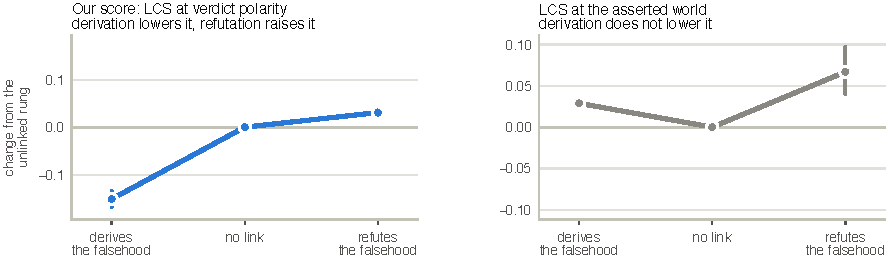
\includegraphics[width=\textwidth]{figures/fig_sign.pdf}
\caption{\textbf{Only the verdict-polarity score orders \cp{sign} as declared.} The
\sThreeNSign{} gold \cp{sign} ladders, rung by rung: each readout's change from the rung that draws
no link, averaged over ladders, with 95\% bootstrap intervals. The declared order is
$\rho_0<\rho_1<\rho_2$, a line rising left to right. Each panel has its own vertical scale.}
\label{fig:sign}
\end{figure*}

\paragraph{Resolution on gold graphs.} Gold $\LCS$ resolves \sThreeGoldLamIncTol{} of the increases. The 17 it does not resolve all lie where
$\LCS$ is below $0.06$ or above $0.9$, where the logistic compresses a step of $0.07$--$0.53$
nats in $\Lambda$ below $\tau$.

\paragraph{Weights and saturation.} The two miners differ most in their weights. The graph-level miner weighs a link by its vote share
times a band midpoint, at most $0.925$, and resolves most increases: \sThreeGraphGptLamIncTol{}
with GPT-6 and \sThreeGraphOssLamIncTol{} with gpt-oss-120b. The pairwise miner weighs a link by
the product of its label and \texttt{Yes} token probabilities, which for a confident model are
nearly $1$: \sThreePairOssWHard{} of gpt-oss-120b's relations and \sThreePairLlamaWHard{} of
Llama's carry a weight of at least $0.99$. A conflict of that weight at the committed world all
but rules that world out, so $\LCS<0.01$ on \sThreePairOssSat{} and \sThreePairLlamaSat{} of their
responses (\sThreeGoldSat{} on gold). The score still orders their rungs, by a median step in
$\Lambda$ of \sThreePairOssStep{} and \sThreePairLlamaStep{} nats, but this close to $0$ the
$[0,1]$ scale compresses these steps below $\tau$: only \sThreePairOssLamIncTol{} and \sThreePairLlamaLamIncTol{} of their increases are
resolved. The weights of Eq.~\ref{eq:decomp} are not calibrated, and near-certain ones turn soft
checks into hard constraints that saturate the score.

\paragraph{Invariance on mined graphs.} It measures how stable the miner is, not the score: A2 promises nothing
about a graph that has changed. GPT-6 returned the same consensus graph for both rungs on
\sThreeGraphGptLamInv{} invariance pairs, and on \sThreeGraphGptLamOrder{} \cp{order} pairs, so
permuting a response's paragraphs changes what it extracts about half the time. gpt-oss-120b,
sampled at temperature $0.7$, rarely returns the same graph (\sThreeGraphOssLamInv), and the pairwise miner, whose weights are token probabilities that shift by about
$10^{-8}$ when any sentence of the response changes, almost never does (\sThreePairOssLamInv{} and
\sThreePairLlamaLamInv). Within $\tau$, GPT-6 keeps \sThreeGraphGptLamInvTol{} invariances. The pairwise arms reach
\sThreePairOssLamInvTol{} and \sThreePairLlamaLamInvTol{}, but that figure is inflated by
saturation: two responses pinned near $\LCS=0$ are trivially within $\tau$ of each other. Tolerant invariance is informative only next to the resolved increases.

\paragraph{Baselines by ladder type.} Table~\ref{tab:baselines} breaks the baselines down by ladder type. Three of them read only the
claims (claim count, NLI contradiction and ROSCOE), which are identical across a family's rungs, so
they tie on every pair: every invariance is kept and no increase is satisfied. The entity graph
reads the entities the text mentions, which an edit almost never changes: it rises on
\sThreeBDiscEGInc{} increases and keeps \sThreeBDiscEGInv{} invariances.
Length and DiscoScore move with the surface of the edit and fall about as often as they rise
(Figure~\ref{fig:ladders}, middle). Length rises with each added link and so passes
\sThreeBCtlLengthChain{} \cp{chain} pairs without reading any logic, the confound a length control
exists to expose; it falls on \sThreeBCtlLengthConflictFalls{} \cp{conflict} pairs, because a
filler that sets two claims against each other is longer than one that does not.

% Generated by scripts/arr_slot3_example.py -- do not edit by hand.
\begin{table*}[t]
\centering\small
\setlength{\tabcolsep}{4pt}
\begin{tabular}{@{}p{3.3cm}p{11.7cm}@{}}
\toprule
\multicolumn{2}{@{}p{15.4cm}@{}}{\emph{Question:} How did astronomers establish whether the ``Great Debate'' nebulae lay within the Milky Way or formed separate galaxies, and what evidence ultimately settled the dispute?} \\
\midrule
Rung & The sentences that differ between the rungs \\
\midrule
$\rho_0$: derives the falsehood & Curtis cited novae observed in spiral nebulae as evidence that those nebulae lay at great distances; that evidence indicates a remove for M31 of about 10,000 light years from the Sun, the figure his analysis of those novae yielded. \\
$\rho_1$: no link & Curtis cited novae observed in spiral nebulae as evidence that those nebulae lay at great distances. His analysis of novae in spiral nebulae placed M31 about 10,000 light years from the Sun. \\
$\rho_2$: refutes the falsehood & Curtis cited novae observed in spiral nebulae as evidence that those nebulae lay at great distances, and that evidence rules out the claim, sometimes attached to his analysis of novae in spiral nebulae, that it placed M31 about 10,000 light years from the Sun. \\
\bottomrule
\end{tabular}

\vspace{4pt}
\begin{tabular}{@{}lcccl@{}}
\toprule
Score & $\rho_0$ & $\rho_1$ & $\rho_2$ & order \\
\midrule
$\LCS$, gold graph (ours) & 0.123 & 0.292 & 0.334 & as declared \\
$\LCS$ at the asserted world, gold graph & 0.036 & 0.030 & 0.036 & partly \\
mean posterior marginal, gold graph & 0.770 & 0.766 & 0.764 & reversed \\
$\LCS$, GPT-6 graph-level miner (ours) & 0.045 & 0.350 & 0.395 & as declared \\
G-Eval judge, GPT-6 & 0.650 & 0.600 & 0.500 & reversed \\
1--5 rating judge, GPT-6 & 0.250 & 0.250 & 0.250 & no change \\
response length & 0.413 & 0.406 & 0.418 & partly \\
\bottomrule
\end{tabular}
\caption{One \cp{sign} ladder of the test split (f003), end to end. The slot joins a true claim (``Curtis cited novae observed in spiral nebulae as evidence that those nebulae lay at great distances.'') and a false one (``Curtis's analysis of novae in spiral nebulae placed M31 about 10,000 light years from the Sun.''). The three rungs share every other sentence of the 406-word answer, every claim and every verdict; only the link between the two claims changes. Judges are means of five runs mapped to $[0,1]$; length is normalized.}
\label{tab:example}
\end{table*}


\paragraph{One ladder, end to end.} Table~\ref{tab:example} shows a \cp{sign} ladder with every
score. On the gold graph $\LCS$ rises at each rung; on the GPT-6 graph-level arm's graphs it rises too. The
score read at the asserted world rates deriving the falsehood and refuting it alike. The G-Eval judge
prefers the rung that derives the falsehood, and the 1--5 rating does not move.

\begin{table*}[t]
\centering\small
\setlength{\tabcolsep}{3.4pt}
\begin{tabular}{@{}ll ccc c cc@{}}
\toprule
& & \multicolumn{4}{c}{Increase} & \multicolumn{2}{c}{Invariance, exact} \\
\cmidrule(lr){3-6}\cmidrule(l){7-8}
Arm & Readout & \cp{conflict} & \cp{chain} & \cp{sign} & resolved & \cp{order} & \cp{control} \\
\midrule
\multirow{2}{*}{\cp{gold}}
 & $\LCS$, assertion & \sThreeGoldLamAConflict & \sThreeGoldLamAChain & \sThreeGoldLamASign & \sThreeGoldLamAIncTol & \sThreeGoldLamAOrder & \sThreeGoldLamAControl \\
 & $\LCS$, verdict (ours) & \sThreeGoldLamConflict & \sThreeGoldLamChain & \sThreeGoldLamSign & \sThreeGoldLamIncTol & \sThreeGoldLamOrder & \sThreeGoldLamControl \\
\midrule
\multirow{2}{*}{graph, GPT-6}
 & $\LCS$, assertion & \sThreeGraphGptLamAConflict & \sThreeGraphGptLamAChain & \sThreeGraphGptLamASign & \sThreeGraphGptLamAIncTol & \sThreeGraphGptLamAOrder & \sThreeGraphGptLamAControl \\
 & $\LCS$, verdict (ours) & \sThreeGraphGptLamConflict & \sThreeGraphGptLamChain & \sThreeGraphGptLamSign & \sThreeGraphGptLamIncTol & \sThreeGraphGptLamOrder & \sThreeGraphGptLamControl \\
\midrule
\multirow{2}{*}{graph, gpt-oss}
 & $\LCS$, assertion & \sThreeGraphOssLamAConflict & \sThreeGraphOssLamAChain & \sThreeGraphOssLamASign & \sThreeGraphOssLamAIncTol & \sThreeGraphOssLamAOrder & \sThreeGraphOssLamAControl \\
 & $\LCS$, verdict (ours) & \sThreeGraphOssLamConflict & \sThreeGraphOssLamChain & \sThreeGraphOssLamSign & \sThreeGraphOssLamIncTol & \sThreeGraphOssLamOrder & \sThreeGraphOssLamControl \\
\midrule
\multirow{2}{*}{pairwise, gpt-oss}
 & $\LCS$, assertion & \sThreePairOssLamAConflict & \sThreePairOssLamAChain & \sThreePairOssLamASign & \sThreePairOssLamAIncTol & \sThreePairOssLamAOrder & \sThreePairOssLamAControl \\
 & $\LCS$, verdict (ours) & \sThreePairOssLamConflict & \sThreePairOssLamChain & \sThreePairOssLamSign & \sThreePairOssLamIncTol & \sThreePairOssLamOrder & \sThreePairOssLamControl \\
\midrule
\multirow{2}{*}{pairwise, Llama}
 & $\LCS$, assertion & \sThreePairLlamaLamAConflict & \sThreePairLlamaLamAChain & \sThreePairLlamaLamASign & \sThreePairLlamaLamAIncTol & \sThreePairLlamaLamAOrder & \sThreePairLlamaLamAControl \\
 & $\LCS$, verdict (ours) & \sThreePairLlamaLamConflict & \sThreePairLlamaLamChain & \sThreePairLlamaLamSign & \sThreePairLlamaLamIncTol & \sThreePairLlamaLamOrder & \sThreePairLlamaLamControl \\
\bottomrule
\end{tabular}
\caption{Ladder assertions on LoCoBench by type (pairs satisfied / pairs). ``Resolved'':
Increase pairs whose $[0,1]$-scale score rises by more than
$\tau=\sThreeTol$, out of \sThreeNIncPairs.}
\label{tab:bytype}
\end{table*}

\begin{table}[t]
\centering\small
\setlength{\tabcolsep}{3.0pt}
\begin{tabular}{@{}lccccc@{}}
\toprule
Arm & F1 & Ordered & Incomp. & Equal & Backward \\
\midrule
\cp{gold} & --- & \sThreeGoldDomForwardPos/\sThreeGoldDomForward & --- & --- & --- \\
graph, GPT-6 & \sThreeGraphGptCoupF & \sThreeGraphGptDomForwardPos/\sThreeGraphGptDomForward
  & \sThreeGraphGptDomIncomparableOk/\sThreeGraphGptDomIncomparable
  & \sThreeGraphGptDomEqualTies/\sThreeGraphGptDomEqual
  & \sThreeGraphGptDomBackwardFalls/\sThreeGraphGptDomBackward \\
graph, gpt-oss & \sThreeGraphOssCoupF & \sThreeGraphOssDomForwardPos/\sThreeGraphOssDomForward
  & \sThreeGraphOssDomIncomparableOk/\sThreeGraphOssDomIncomparable
  & \sThreeGraphOssDomEqualTies/\sThreeGraphOssDomEqual
  & \sThreeGraphOssDomBackwardFalls/\sThreeGraphOssDomBackward \\
pair., gpt-oss & \sThreePairOssCoupF & \sThreePairOssDomForwardPos/\sThreePairOssDomForward
  & \sThreePairOssDomIncomparableOk/\sThreePairOssDomIncomparable
  & \sThreePairOssDomEqualTies/\sThreePairOssDomEqual
  & \sThreePairOssDomBackwardFalls/\sThreePairOssDomBackward \\
pair., Llama & \sThreePairLlamaCoupF & \sThreePairLlamaDomForwardPos/\sThreePairLlamaDomForward
  & \sThreePairLlamaDomIncomparableOk/\sThreePairLlamaDomIncomparable
  & \sThreePairLlamaDomEqualTies/\sThreePairLlamaDomEqual
  & \sThreePairLlamaDomBackwardFalls/\sThreePairLlamaDomBackward \\
\bottomrule
\end{tabular}
\caption{Increase pairs by how the two rungs' extracted graphs compare in the coherence order at
the verdicts (the counts behind Figure~\ref{fig:dominance}). Ordered: pairs on which $\LCS$ rises / pairs,
by the exact sign of the change, as the theorem states it (on one pairwise-Llama pair the rise is
$4\times10^{-14}$ in $\Lambda$, below the $10^{-9}$ at which Table~\ref{tab:ladders} counts an
increase; \S\ref{sec:exp-mined}). Incomparable: pairs on which it rises by more than $10^{-9}$ /
pairs. Equal: pairs on which it ties; backward: pairs on which it falls,
as the theorem requires. F1: coupling-level extraction F1.}
\label{tab:dominance}
\end{table}

\paragraph{Gold ladders.} Averaged over the \sThreeNConflict{} ladders of each primary type
(\sThreeNControl{} for \cp{control}), gold $\LCS$ rises from
\sThreeGoldConflictLcsA{} to \sThreeGoldConflictLcsB{} to \sThreeGoldConflictLcsC{} on \cp{conflict},
from \sThreeGoldChainLcsA{} to \sThreeGoldChainLcsB{} to \sThreeGoldChainLcsC{} on \cp{chain} and
from \sThreeGoldSignLcsA{} to \sThreeGoldSignLcsB{} to \sThreeGoldSignLcsC{} on \cp{sign}, and stays
at \sThreeGoldOrderLcsA{} on \cp{order} and \sThreeGoldControlLcsA{} on \cp{control}.

\paragraph{Extraction quality.} Pair-level precision/recall/F1 of the mined arms against gold
(relations with a factor) is \sThreeGraphGptPairP/\sThreeGraphGptPairR/\sThreeGraphGptPairF{}
(graph, GPT-6), \sThreeGraphOssPairP/\sThreeGraphOssPairR/\sThreeGraphOssPairF{} (graph,
gpt-oss-120b), \sThreePairOssPairP/\sThreePairOssPairR/\sThreePairOssPairF{} (pairwise,
gpt-oss-120b) and \sThreePairLlamaPairP/\sThreePairLlamaPairR/\sThreePairLlamaPairF{} (pairwise,
Llama-3.3-70B); coupling-level F1 is \sThreeGraphGptCoupF, \sThreeGraphOssCoupF, \sThreePairOssCoupF{}
and \sThreePairLlamaCoupF. The arms average \sThreeGraphGptRels, \sThreeGraphOssRels,
\sThreePairOssRels{} and \sThreePairLlamaRels{} factor-bearing relations per response, against
\sThreeGoldRels{} in gold.

\paragraph{Judges within their own spread.} Counting an invariance pair as satisfied when the two
means differ by no more than the larger of their five-run standard deviations, the judges reach
\sThreeBGevalGptInvTol{} (G-Eval, GPT-6), \sThreeBGevalOssInvTol{} (G-Eval, gpt-oss-120b),
\sThreeBDirectGptInvTol{} (rating, GPT-6) and \sThreeBDirectOssInvTol{} (rating, gpt-oss-120b).
The five runs are independent samples. The gateway that serves GPT-6 caches identical requests and
would otherwise answer all five from the first completion; a first run with the cache on had zero
spread on every response, and it is not reported.

